\chapter[Publicação]{Publicação}
\section{Visão Geral}
O intuito dessa seção é documentar todo o processo de publicação dos três componentes essênciais, a API dicionário, API principal e o aplicativo móvel. Dessa forma, deixamos claro todos os passos e requisitos para ter o sistema Agromart rodando e funcionando em ambientes de produção, acessível ao público através da loja de aplicativos da Google.

\subsection{Nome do aplicativo e do pacote java}
Nosso objetivo nesse trabalho a nível de publicação foi corrigir os defeitos necessários para termos um MVP rodando, e públicar esse MVP custeando o valor dos servidores, e de forma com que essa publicação na interfira com publicações futuras do Agromart. Por isso decidimos publicar o aplicativo em uma conta pessoal, uma vez que ele não funcionará mais uma vez que deixarmos de custear os servidores, e será removido da loja.

O nome do pacote deve ser único para cada aplicativo publicado na Google Play Store, por isso, utilizamos o nome de pacote  \texttt{com.tcc.agromart} para gerar as builds do aplicativo, e não o nome de pacote padrão do Agromart que é \texttt{com.agromart}, dessa forma, o nosso deploy não interfere na publicação de outras versões futuras do Agromart em outras contas.

O nosso publicado com o nome Agromart - CT, onde CT significa Christian e Thiago, que foi usado para diferenciar o aplicativo da publicação oficial que será feita através de constas gerenciadas pela instituição UnB.

\section{Processo de deploy do servidores}
A motivação de realizarmos a publicação dos servidores foi a necessidade de ambientes reais rodando, acessíveis via HTTPS, para que a versão de produção do aplicativo e que pudesse ser devidamente publicada na Google Play Store, uma vez que os aplicativos publicados passam por revisão manual. Sendo assim o aplicativo só poderia ser aprovado na loja se estivesse se comunicando com servidores reais e persistindo dados corretamente.

\subsection{Serviço escolhido}
O Amazon EC2 (Elastic Compute Cloud) é um serviço de computação em nuvem da AWS (Amazon Web Services) que permite aos usuários criar máquinas virtuais em nuvem com diferentes configurações de CPU, memória, armazenamento e rede. Essas instâncias podem rodar sistemas operacionais, aplicativos e outros serviços, permitindo que você execute cargas de trabalho como se estivesse utilizando servidores físicos, mas com a flexibilidade e escalabilidade da nuvem. Essas configurações podem ser facilmente manipuladas de acordo com a necessidade do usuário.

A principal razão para a escolha da EC2 na realização do deploy dos servidores foi a flexibilidade que o serviço oferece para modificar os recursos da instância alocada. Sem saber inicialmente quanto recurso seria necessário para o bom funcionamento do Agromart, a escolha de uma opção que permitisse a fácil manipulação dos recursos computacionais foi fundamental.

Levando em conta as necessidades listadas, foi alocada uma instância EC2 na AWS para disponibilizar a API Dicionário e o Backend do Agromart. A instância EC2 selecionada possui as seguintes características: tipo de instância t3.medium, com 2 vCPUs, 4 GB de memória RAM, e um volume de armazenamento de 30 GB em um SSD como visto na Fig. \ref{ec2}. O sistema operacional escolhido foi o Linux, e a instância foi alocada na região da AWS da Virgínia do Norte (us-east-1).

Adicionalmente, também foram criados snapshots do volume para recuperar o estado dos servidores em caso de falha. A configuração foi realizada com o objetivo de balancear adequadamente o custo e o desempenho.

\begin{figure}[h]
        \centering
        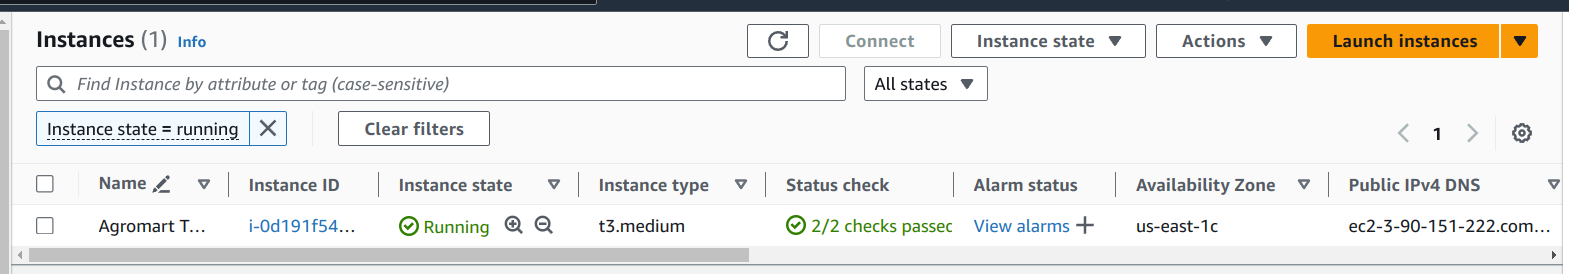
\includegraphics[keepaspectratio=true,scale=0.3]{figuras/ec2_agromart.png}
        \caption{Imagem da EC2 do Agromart}
        \label{ec2}
\end{figure}

\subsection{Preparação do Banco de Dados}
Para a preparação do banco de dados, foi utilizado o SGBD PostgreSQL. A imagem oficial do PostgreSQL foi usada para criar o banco de dados em um ambiente Docker. Essa abordagem foi escolhida por ser uma forma rápida de instalar e rodar o banco de dados no servidor.

\subsection{Aquisição de Domínio}
Um domínio foi essencial para conseguirmos um certificado SSL válido, que por sua vez é necessário para que possamos habilitar o HTTPS em nosso servidores. O domínio foi comprado através da plataforma Hostinger, e seu endereço é agromarttcc.shop, por um prazo de 1 ano, conforme apresentado na Fig. \ref{dominio}. 

\begin{figure}[h]
	\centering
	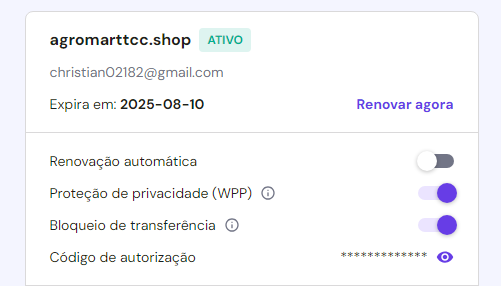
\includegraphics[keepaspectratio=true,scale=0.35]{figuras/dominio.png}
	\caption{Visualização do domínio na plataforma Hostinger}
	\label{dominio}
\end{figure}

\subsection{Configuração de HTTPS, domínio e certificado}
HTTPS (Hypertext Transfer Protocol Secure) é uma versão segura do protocolo HTTP, usado para a comunicação entre navegadores web e servidores. A principal diferença é que o HTTPS criptografa os dados enviados e recebidos, garantindo maior segurança das informações transmitidas.

No caso do Agromart, disponibilizar nossos servidores através de HTTPS é extremamente necessário, pois chamadas puramente HTTP não são permitidas em aplicativos publicados na Google Play Store.

O Nginx é uma ferramenta para servidores web poderosa e muito utilizada, no contexto do Agromart, utilizamos o Nginx como Proxy Reverso dos nossos servidores (CSAs implantadas e API dicionário). Dessa forma todas chamadas feitas aos nossos servidores passam primeiro pelo Nginx, que encaminha para o servidor correto. O proxy reverso com Nginx também permitiu a implementação de certificados SSL que era necessário para o protocolo HTTPS.

 O certificado SSL necessário para habilitar o HTTPS foi obtido gratuitamente através da ferramenta Certbot, que nos proveu um certificado para o domínio agromarttc.shop.

 Com todas essas configurações feitas, a única coisa restante foi apontar o nosso domínio para o IP público da nossa máquina virtual onde os servidores estavam rodando, esse processo foi feito pelo painel da Hostinger.

\section{Processo de deploy do Aplicativo na Google Play Store}

\subsection{Conta no Expo e EAS}
O Aplicativo do Agromart foi criado utilizando uma ferramenta chamda Expo. O Expo é uma plataforma de desenvolvimento de aplicativos com React Native, que foi a tecnologia escolhida para o aplicativo em sua idealização.

o EAS (Expo Application Services) é um conjunto de ferramentas para deploy de aplicativos que utilizam o Expo. Utilizamos o serviço EAS Build, que permite compilar e gerar buils para Android na núvem, sem necessidade de instalação de ferramentas para compilação localmente.

Para isso, foi criada uma conta do Expo específica para esse projeto de conclusão de curso, para build da versão de produção que foi sumetida à Google Play Store. Na figura \ref{expo}, podemos ver a conta no Expo e algumas das builds de produção geradas.

\begin{figure}[h]
	\centering
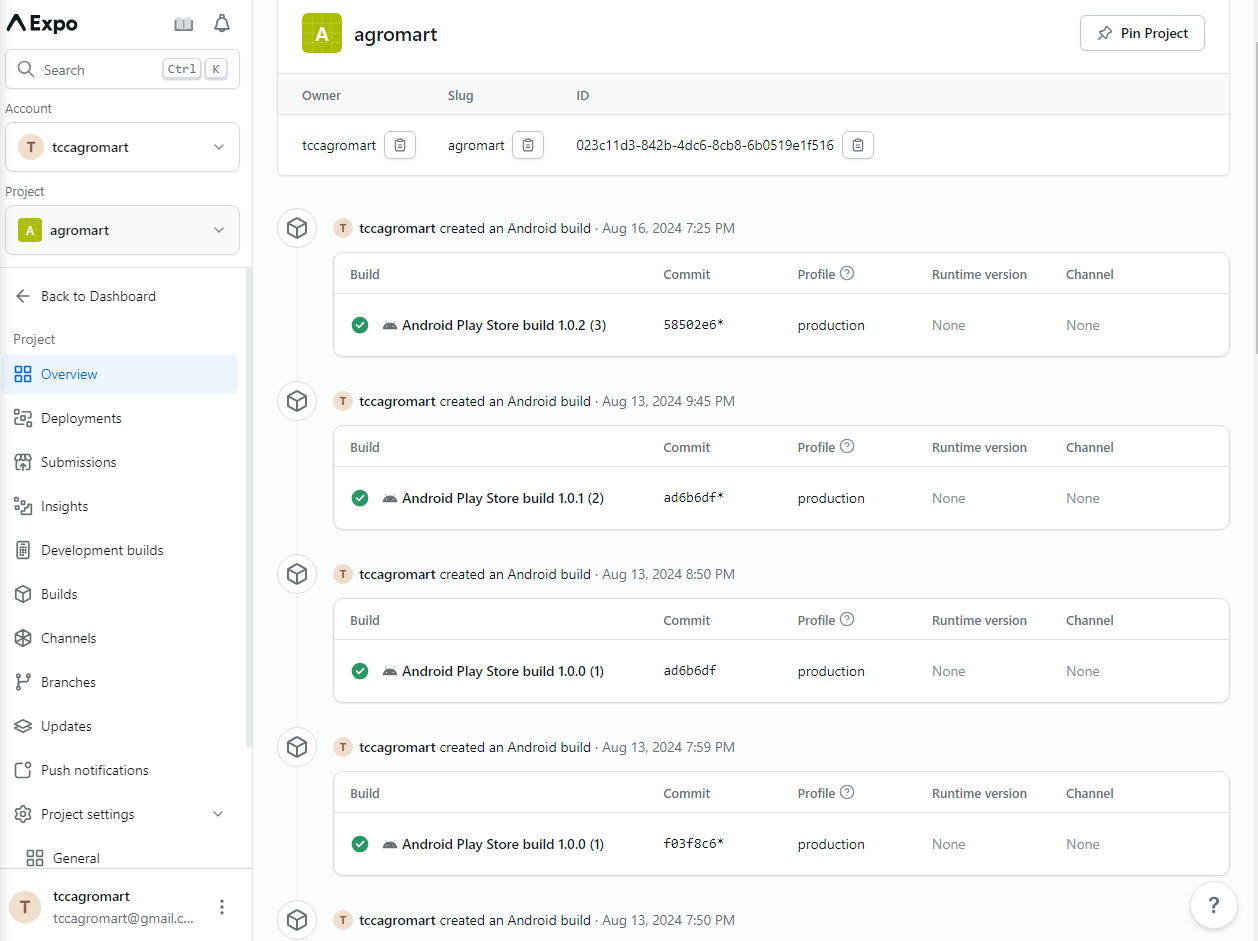
\includegraphics[keepaspectratio=true,scale=0.35]{figuras/expo.png}
	\caption{Painel da conta Expo com Builds realizadas}
	\label{expo}
\end{figure}

\subsection{Geração de Builds de produção}

Uma build de produção é uma versão de um software que está pronta para ser lançada e usada pelos usuários finais. Após a correção de diversos defeitos, pudemos enfim concluir que tinhamos atingindo já um MVP do Agromart, e gerar nossa primeira build de produção.

Após isso, executamos o comando \texttt{eas build  ---profile production  ---platform android.} Esse comando dispara a compilação em núvem, gerando um arquivo .aab, que é o o arquivo que devemos submeter à Play Store.

\subsection{Conta de Desenvolvedor da Google Play Store}
Para publicar aplicativos da Google Play Store, é necessário fazer um registro na plataforma Google Play Console e pagar uma taxa única de 25\$, para isso, utilizamos uma conta de desenvolvedor que já havia sido adquirida anteriormente por um dos realizadores deste trabalho.

\subsection{Versão de teste interno}
O Google Play Console disponibiliza a possibilidade de serem publicadas versões para testes internos. Essas versões permitem os desenvolvedores lançar versões preliminares de seus aplicativos para um grupo restrito de usuários antes do lançamento oficial. Essa versão é ideal para realizar testes iniciais com um número limitado de testadores confiáveis, como membros da equipe de desenvolvimento, além de que não passa por uma revisão como a versão de produção, e podemos fazer uma publicação quase imediata. Através do teste interno, os desenvolvedores podem identificar e corrigir problemas, como defeitos e crashes. Os testadores são selecionados através de uma lista de endereços de email, e os dois autores deste trabalho foram incluidos nessa lista. Isso possibilitou que identificássemos um crash crítico ao abrir o Agromart que ocorria apenas em builds de produção.

\subsection{Configuração do Aplicativo na Google Play Store e Publicação}
É necessário a criação de um novo aplicativo através do painel do Play Console, e após isso fazer o upload do arquivo de build gerado, criando assim uma nova versão do aplicativo.
Após isso, é necessário fazer uma configuração detalhada do aplicativo para enviar para revisão. Como visto na Na figura \ref{app-conf}, há uma serie de informações obrigatórias como público alvo, recursos financeiros e política de privacidade. A política de privacidade foi gerada através de ferramentas online e está disponível em \href{https://www.freeprivacypolicy.com/live/b43f2c89-15ae-43e1-a55b-d3eec294da3b}.
.


\begin{figure}[h]
	\centering
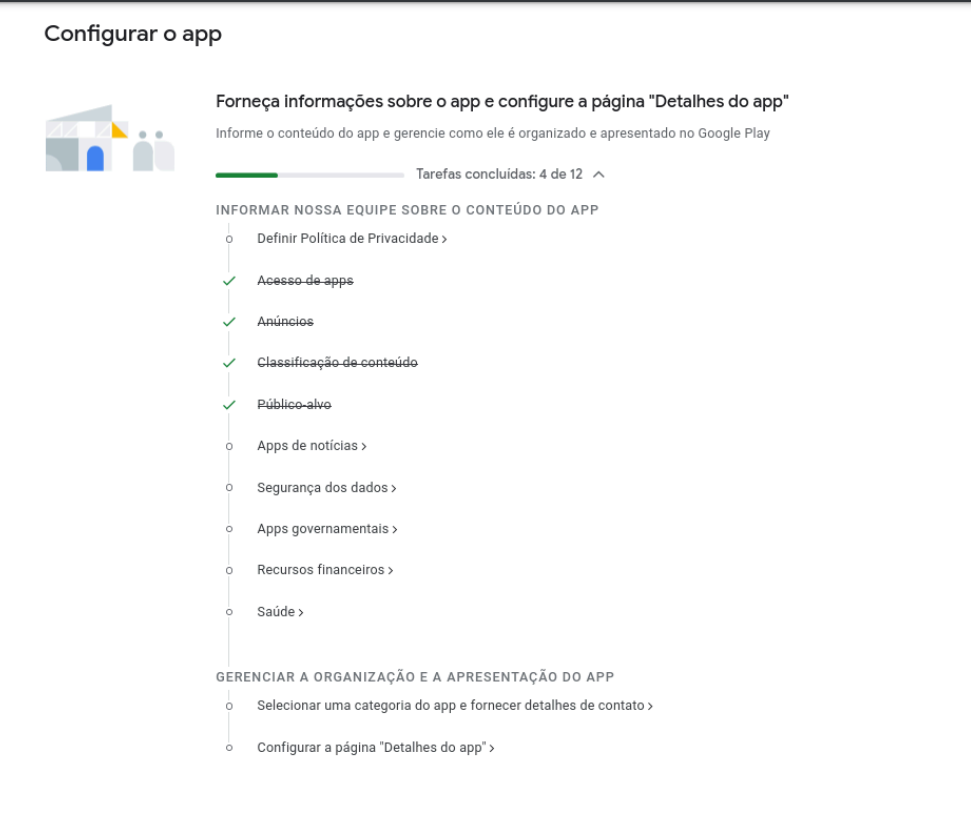
\includegraphics[keepaspectratio=true,scale=0.35]{figuras/app-conf.png}
	\caption{Configuração do aplicativo no Play Console}
	\label{app-conf}
\end{figure}


Além disso, antes de enviar o aplicativo para revisão é necessário criar as instruções necessárias para o acesso ao aplicativo, uma vez que, de acordo com as políticas do Google, um revisor não pode criar contas nos aplicativos que irá revisar. Dessa forma, é necessário prover uma conta válida e instruções gerais de como se logar no aplicativo. 

\begin{figure}[h]
	\centering
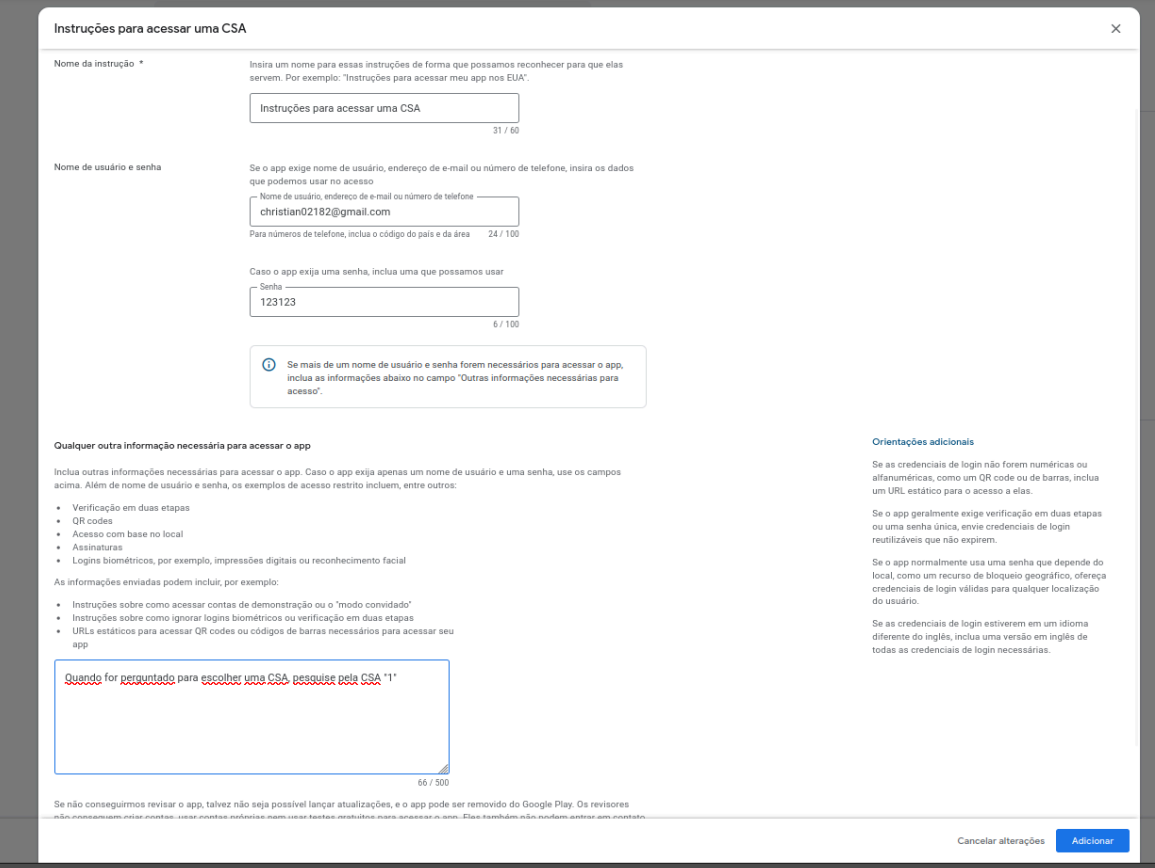
\includegraphics[keepaspectratio=true,scale=0.35]{figuras/login-inst.png}
	\caption{Formulário de instruções de login}
	\label{login-inst}
\end{figure}

Após esse processo, o aplicativo pode ser submetido à revisão, e em um prazo de 7 dias úteis, será públicado na Google Play Store ou, caso haja alguma pendência, gerado um alerta pra que sejam feitas correções no aplicativo antes de uma próxima revisão.

Nosso aplicativo foi aceito e encontra se disponível em  \href{https://play.google.com/store/apps/details?id=com.ct.agromart}{Agromart - CT}.
